\section{Orientierungen im Informationsmanagement - OS}

Hochschulen befinden sich bei der Bereitstellung von Informationssystemen in einem stetigen Entwicklungsprozess. Ihnen stehen dabei drei grundlegende Orientierungen zur Verfügung: Serviceorientierung, Prozessorientierung und Architekturorientierung.\footcite[Vgl.][32]{leitner_itil_2008} Kapitel \ref{subsection_serviceorientierung} geht dabei auf die Bedeutung und Umsetzungsmöglichkeiten der Serviceorientierung ein. 

Kontinuierlich verbesserte Prozesse und Gestaltungen von IT-Strukturen werden im Kapitel \ref{subsection_prozessorientierung} behandelt. Die Architekturorientierung wird hier nicht betrachtet, Kapitel \ref{subsubsection_gestaltung_IT_strukturen} geht allerdings grundlegend auf Architekturveränderungen in der IT-Infrastruktur ein. In einer Konklusion werden die Service- und Prozessorientierung am Ende gegenübergestellt und miteinander verglichen.


\subsection{Serviceorientierung}
\label{subsection_serviceorientierung}
Die zentralen Ziele der Serviceorientierung liegen darin, die Dienstleistungen auf die 
Anforderungen der Kunden auszurichten und dabei gleichzeitig ihre Qualität kontinuierlich 
zu verbessern. Kundenorientierung bedeutet weiter, die bestehenden und zukünftigen 
Kundenbedürfnisse zu kennen, die Interessen zu berücksichtigen und in den Mittelpunkt zu 
stellen.\footcite[Vgl.][34]{leitner_itil_2008} Die Herausforderung dieser Ambition liegt bei 
erstmaligem Betrachten in den technologiefokussierten IT-Abteilungen der Hochschule, die 
es in kundenorientierte IT-Dienstleister zu verwandeln gilt. Hochschulrechenzentren 
verstehen sich dabei als zentrale, wissenschaftliche Dienstleistungseinrichtung für 
öffentliche Hochschulen.\footcite[Vgl.][10]{schroeder_2011} Zusätzlich hindern 
wissenschaftliche Ambitionen des IT-Personals die Realisierung kundenorientierter 
Serviceangebote. Andererseits verbindet die Forschung wieder die Hochschulrechenzentren 
mit Ihren Kunden. Erschwerend kommt hinzu, dass die Rollenverteilung in Hochschulen 
zwischen Kunden und Dienstleistern nicht klar definiert werden kann. Die unterschiedlichen 
Serviceorganisationen der Hochschule sind der Rolle der Dienstleister zuzuordnen. Auf 
Seiten der Kundensicht kommen Studierende, Hochschulen selbst, aber auch ihre Fakultäten, 
Fachbereiche, die Lehrenden und Verwaltungsmitarbeiter in Frage. Trotz alledem ist eine 
stärkere Serviceorientierung aufgrund steigenden Wettbewerbs um Studierende und 
potenziellen Forscher-Nachwuchs, veränderten Auswahlverhaltens und gestiegenem 
Anspruchsdenken der Studierenden notwendig.\footcite[Vgl.][14]{leitner_itil_2008}

\subsubsection{Realisierung der Serviceorientierung}
\label{realisierung_der_serviceorientierung}
Um das Wertversprechen gegenüber Studierenden weiter zu verbessern, ist die Optimierung der Serviceorientierung wichtig. Erreicht werden könnte dies beispielsweise durch eine Verbesserung der Bibliotheksangebote und weitreichendere Öffnungszeiten. Darüber hinaus können mittels verbesserter Lehrqualität neue berufs- und ergebnisorientierte Bedürfnisse der Studierenden befriedigt werden. Weiter lässt sich durch eine stärkere Einbindung von Praktikern als Gastdozierende und Mentoren praxisrelevantes Wissen vermitteln. Eine reibungslose Abwicklung und große Auswahl an institutionalisierten Austauschprogrammen und Auslandssemestern ist ebenfalls förderlich. Die individualisierte Karriereförderung sollte allerdings über die eigentliche Studienbetreuung hinaus gehen und personalisierte Bewerbungstrainings und Karrierecoachings, sowie persönliche Kontakte zu Arbeitgebern beinhalten. Um mit potentiellen Arbeitgebern frühzeitig in Kontakt treten zu können, sind Career Services und der Ausbau von Jobmessen wichtig.\footcite[Vgl.][13]{schroeder_2011}

Verbesserte Dienstleistungen werden von Studierenden hoch geschätzt. So ist besonders für berufstätige Studierende eine flexible Lehre wichtig. Dazu gehören ergänzend zum Präsenzunterricht E-Learning-Angebote (siehe Kapitel \ref{subsubsection_e_learning_plattformen}) aber auch Verfahrensweisen wie BYOD (siehe Kapitel \ref{netzinfrastruktur_consumerization_und_byod}). Serviceorientierung lässt sich weiter durch effiziente Gestaltung von Bewerbungsverfahren und bedienerfreundlichem Kursauswahlverfahren erzielen. \footcite[Vgl.][18]{deutsche_wissenschaft_2010}

Große Systemvielfalt beinhaltet viele Login-Prozesse und unterschiedliche Ansprechpartner. Hier ist das Ziel weniger Systeme  und mehr Serviceorientierung einzusetzen, um eine bessere Nutzerfreundlichkeit zu erreichen. Durch ein SSO (Single Sign-On) wird nach einer einmaligen Anmeldung an einem Portal wie in Abbildung \ref{fig_sso} dargestellt, ein genereller Zugriff auf alle Anwendungen gewährt. So können Tätigkeiten wie beispielsweise Prüfungsanmeldungen, Zugriffe auf Rechenzentren, Bibliotheken oder die Verwaltung mit nur einem Login durchgeführt werden.\footcite[Vgl.][81]{deutsche_wissenschaft_2010}

\begin{figure}[h!]
	\centering
	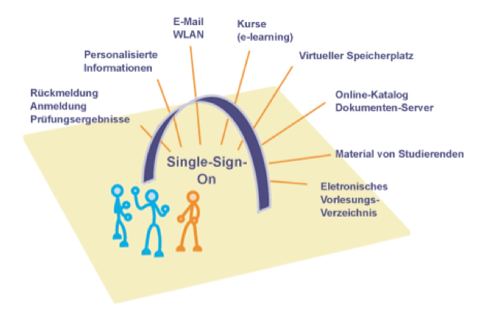
\includegraphics[width=10cm]{kapitel/gruppe1_2/bilder/SSO}
	\caption{Single-Sign-On\protect\footnotemark}
	\label{fig_sso}
\end{figure}\footnotetext{\cite[81]{deutsche_wissenschaft_2010}}


\subsubsection{IT Infrastructure Library (ITIL)}
\label{subsubsection_ITIL}
Zur Fokussierung der IT-Dienste auf Kundenorientierung und für eine stärkere Ausrichtung des 
IT-Bereichs an strategischen Organisationszielen, stehen Hochschulen und anderen Institutionen 
verschiedene Referenzmodelle zur Verfügung. Diese Modelle unterstützen bei der Bereitstellung klar 
definierter IT-Services, einer kennzahlengestützten Steuerung und Bewertung des IT-Managements und 
Umstrukturierung der IT-Organisation. Die IT Infrastructure Library (kurz ITIL) ist das international am 
meisten genutzte Referenzmodell. Es ist aus einer Sammlung von Beispielen guter Praxis entstanden 
und wird stetig weiterentwickelt. In ITIL werden sämtliche Prozesse in Beziehung zueinander gesetzt 
und definiert. Dazu gehören beispielsweise Konfigurationsmanagement, Kapazitäts-, Verfügbarkeits- 
und Finanzplanung, der Umgang mit Katastrophen, Störungs- und Problembehandlung, aber auch 
Service Level Vereinbarungen. ITIL ist durch seine Skalierbarkeit und Prozessorientierung auf 
Gesamtorganisationen, einzelne Abteilungen oder übergreifende Dienstleistungen anwendbar. Die 
Prozesse können unabhängig von einer konkreten IT-Infrastruktur genutzt werden, wodurch der 
Einsatz in vielen Bereichen ermöglicht wird. \footcite[Vgl.][34]{leitner_itil_2008}

\paragraph{Servicedesk}\mbox{}\\\\	

\label{subsubsection_service_desk}
Die Schaffung eines Servicedesks resultiert aus dem Verständnis, die Studierenden und Lehrenden als 
„Kunde“ zu betrachten, denen man serviceorientierte Dienstleistungen anbieten möchte. Zum anderen 
wird eine effizientere Ressourceneinsatzplanung im Verwaltungsbereich ermöglicht. Der Servicedesk ist 
die zentrale Anlaufstelle für jegliche Belange. Hier wird im Zuge des 1st Level Supportes eine Lösung 
der Anfrage ohne Kontaktierung weiteren Fachpersonals versucht. Zusätzlich stellt diese Ebene eine 
schnelle Reaktionszeit bei Störungen sicher. Sollte eine Sofortlösung nicht möglich sein, werden die 
Anfragen über ein Ticketsystem sortiert, priorisiert und den entsprechenden Bearbeitern zugeteilt. Hier 
wird die Bearbeitung zeitversetzt durch Spezialisten im 2nd Level Support fortgeführt. In der Abbildung 
\ref{fig_service_desk} ist der beschriebene Ablauf visualisiert, es handelt sich hier um die Infrastruktur 
der Universität Freiburg. \footcite[Vgl.][5]{klug_2008}

\begin{figure}[h!]
	\centering
	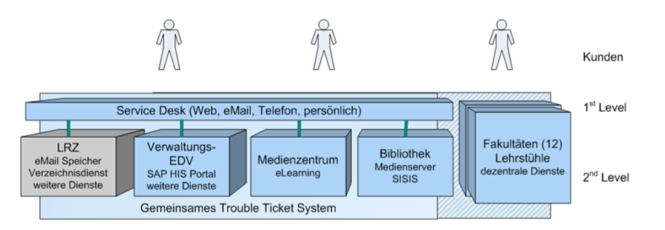
\includegraphics[width=\textwidth]{kapitel/gruppe1_2/bilder/ServiceDesk}
	\caption{Servicedesk: Beispiel an der Universität Freiburg\protect\footnotemark}
	\label{fig_service_desk}
\end{figure}\footnotetext{\cite[15]{bode_2007}}
\newpage

\paragraph{Change-Management}\mbox{}\\\\
Change-Management ist einer der ITIL-Prozesse und beschreibt wie auf Änderungsanfragen zu reagieren ist. Dabei durchläuft der Change (die Veränderung) nachfolgende feingranulare Aktivitäten:

\begin{enumerate}
	\item Change wird erfasst und klassifiziert
	\item Change wird bewertet und freigegeben
	\item Change wird bei Bedarf eskaliert
	\item Change wird implementiert
	\item Change wird getestet und abgenommen
	\item Change wird abgeschlossen
\end{enumerate}

Innerhalb dieses Prozesses gibt es die Rolle des Change Requestors, der die Anfrage stellt. Diese wird 
idealerweise an einer einzigen Stelle wie den Servicedesk aufgegeben, um sicherzustellen, dass alle 
Anforderungen vollständig erfasst und zentral gebündelt sind. Der Change Manager klassifiziert den 
Change und plant die Durchführung. Eine Beurteilung der Änderungsanfrage erfolgt anhand einer 
hochschulweiten vereinbarten Einstufung, die eine Klassifizierung nach Change-Typen vorsieht. In der 
Tabelle \ref{tab_typen_von_changes} sind hier die Change-Typen \glqq Normal Change\grqq, \glqq 
Security Change\grqq und \glqq Notfall Change\grqq als Beispiel aufgeführt, wobei nur im Notfall eine 
Freigabe durch den Change Manager notwendig ist. Der Change Builder setzt die Veränderung 
letztendlich um und der Change Approver prüft und testet die Änderung. 
\footcite[Vgl.][48]{breiter_implementierung_2011}

\begin{table}[h!]
	\begin{tabularx}{\textwidth}{|X|X|X|}
		% Überschriften
		\hline \textbf{Change-Typ} & \textbf{Beschreibung} & \textbf{Genehmigung}\\
		% Zeile 1
		\hline Normal Change & Normalfall & keine Genehmigung durch den Change Manager\\ 
		% Zeile 2
		\hline Security Change & Änderungen für einen bestimmten Anwenderkreis & keine Genehmigung 			durch den Change Manager\\
		% Zeile 3
		\hline Notfall Change & Sofortige Freigabe und Bearbeitung & Genehmigung durch Change 				Manager nötig\\
		\hline
	\end{tabularx}
	\caption{Typen von Changes\protect \footnotemark}
	\label{tab_typen_von_changes}
\end{table}\footnotetext{\cite[48]{breiter_implementierung_2011}}

\paragraph{Service Level Agreements}\mbox{}\\\\
„Service Level Agreements“ (SLAs) sind verbindliche Vereinbarungen zwischen dem Leistungsempfänger 
und dem Leistungserbringer. Die SLAs sichern die Bereitstellung von IT-Dienstleistungen, regeln die 
Dienstleistungsqualität und definieren die Preise für die Erbringung von Leistungen. Weiter werden auch 
Reaktionszeiten je nach Schweregrad definiert und Konventionalstrafen für den Fall von einer 
Überschreitung festgelegt. Betriebszeiten und Ausfallsicherheit wichtiger Infrastruktur sind ebenfalls 
Bestandteile solch einer Vereinbarung.
Zusammengefasst sind SLAs für Dienstleistungsempfänger ein wichtiges Instrument zur Sicherheit und 
Kenntnisnahme über den Leistungsumfang, die Leistungskosten, die minimale Leistungserbringung 
und der benötigten Reaktionszeit. Informationsmanager nehmen hierbei eine beratende Rolle ein und 
unterbreiten zusätzlich Vorschläge zur fachlichen Beschreibung von Zielvorgaben. 
\footcite[Vgl.][499]{heinrich_stelzer_2011}


\subsubsection{Chief-Information Officer (CIO)}
\label{subsubsection_cio}
Der Chief Information Officer (CIO) ist die Berufsbezeichnung für eine Person/Führungskraft, die 
verantwortlich für die Informationstechnik und Anwendungen einer Hochschule ist. 
\footcite[Vgl.][]{beuschel_2009}

\paragraph{Aufgaben und Funktionen des Informationsmanagers}\mbox{}\\\\
\label{aufgaben_funktionen_informationsmanager}
Die Aufgaben des CIO bestehen in der Entwicklung einer IT-Infrastruktur-Strategie und der Ausrichtung der IT auf die Unternehmensstrategie. Seine Tätigkeiten lassen sich im operativen Geschäft auf 3 Kernaufgaben festlegen: 
\begin{enumerate}
	\item Das Planen und Implementieren von Software- und Hardware-Architekturen 
	\item Priorisierung neuer Steuerungsprozessen, sowie neuer Anwendungen
	\item Bereichsübergreifende Koordination
\end{enumerate}

Im Rahmen des Plan-Do-Check-Act-Zyklusses (PDCA), der im Kapitel  \ref{subsubsection_kontinuierlicher_verbesserungsprozess} näher erläutert wird,  sollte er strategische Vorschläge unterbreiten, wie Informationen zur Zielerreichung und Gewinnmaximierung innerhalb der Hochschule eingesetzt werden können. Außerdem hat er Informationen auf die Hochschulkultur und –praxis  abzustimmen und unter Berücksichtigung all dieser Aspekte individuell passende und benutzerfreundliche Werkzeuge auszuwählen. In seiner Verantwortung steht, dass erfolgsentscheidendes Wissen auch in schwierigen Situationen und bei hoher Fluktuation in der Hochschule erhalten bleibt. Organisationen, die über einen CIO mit solch einem Aufgabenprofil verfügen, sind selten. Sie sind eher in modernen Großkonzernen oder Unternehmen mit einer besonderen Affinität zu internetgestützter Kommunikation vorzufinden. \footcite[Vgl.][404]{becker_gora_uhrig_2012}

Aus dieser Aussage lässt sich für deutsche Hochschulen ableiten, dass der Einsatz eines CIOs gut überlegt sein muss. Kleine Hochschulen besitzen einen geringeren Kommunikationsbedarf, als große Hochschulen. Daher ist der Nutzen eines CIOs im Vorfeld gut zu prüfen. Das Kapitel \ref{section_einsatz_cio} wägt den Einsatz eines CIOs für die Hochschule Emden/Leer ab.

\paragraph{Anforderungsprofil}\mbox{}\\\\
\label{anforderungsprofil_informationsmanager}
Ein gutes Anforderungsprofil eines CIOs umfasst eine Mischung aus technischem Wissen, unternehmerischer Denkensweise und Managementfähigkeiten. Für die erfolgreiche Arbeit sind konzeptionelle und analytische Befähigungen aber auch Schlüsselqualifikationen wie Entscheidungsstärke, Organisationstalent, Teamfähigkeit, Führungsqualifikation, Kontaktfähigkeit, Kenntnisse im Projektmanagement und  in der strategischer Planung wichtig. In Abbildung \ref{efec} sind außerdem persönliche Merkmale wie Sensibilisierung und soziales Kompetenzwissen als Erfolgsfaktoren für einen CIO aufgeführt. Die Beziehungen zum CEO und ein Aufbau einer gemeinsamen Vision sind ausschlagegebend für die erfolgreiche Arbeit. Entscheidend ist auch das glaubwürdige Auftreten innerhalb der Hochschule.\footcite[Vgl.][150]{krcmar_einfuhrung_2015}

\begin{figure}[h!]
	\centering
	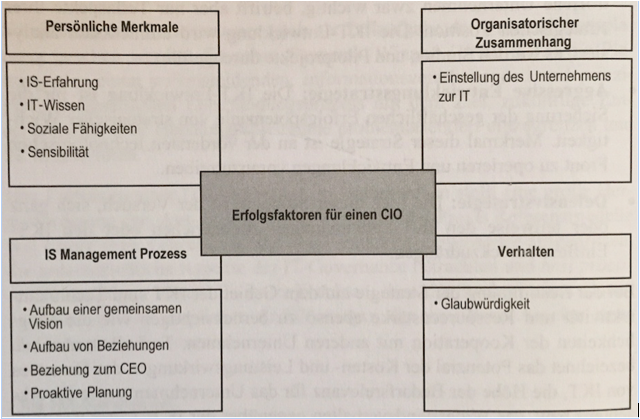
\includegraphics[width=15cm]{kapitel/gruppe1_2/bilder/erfolgsfaktoren_cio} 
	\caption{Erfolgsfaktoren für einen CIO\protect\footnotemark}
	\label{efec}
\end{figure}\footnotetext{\cite[150]{krcmar_einfuhrung_2015}}

\paragraph{Eingliederung in die Hochschulhierarchie}\mbox{}\\\\
Nachdem die grundsätzlichen Aufgaben eines Informationsmanagers erläutert wurden, ist noch die Ansiedlung dieses Postens innerhalb der Hochschulhierarchie zu klären. Das Spektrum reicht hier vom CIO mit Leitungsfunktion repräsentiert durch einen Vizepräsident bis hin zu einer kollektiven Teilung innerhalb des Lenkungsausschusses durch mehrere Personen. Im Detail wird hierauf in Kapitel \ref{subsubsection_zki} eingegangen, insgesamt werden 4 verschiedene Umsetzungstypen unterschieden. \footcite[Vgl.][10]{leitner_itil_2008}

\subsection{Prozessorientierung}
\label{subsection_prozessorientierung}
Die Prozessorientierung ist ein grundlegendes Konzept des Geschäftsprozessmanagements, worunter 
die Gestaltung, Ausführung und Beurteilung von Prozessen verstanden wird. Ein Prozess ist eine 
zusammenhängende Abfolge von Einzelfunktionen, zwischen denen logische Verbindungen bestehen, 
wie in Abbildung \ref{fig_aufgaben_vs_prozess} mit Pfeilen visualisiert wurde. 
\footcite[Vgl.][60]{krcmar_einfuhrung_2015} Weiter lässt sich aus der Abbildung anhand des 
Organigramms ablesen, dass die Gliederung der IT-Organisation an Hochschulen oft funktional 
aufgestellt ist, konkret zu erkennen an dem Netzwerk- und Systembetrieb, Nutzersupport (Servicedesk) 
oder dem Anwendungsmanagement. Diese Aufgabenorientierung erlaubt eine stärkere Spezialisierung 
in den jeweiligen Fachgebieten der Mitarbeiterinnen und Mitarbeiter, widerspricht aber dem Gedanken 
einer Prozessorientierung. Hier ist daher eine klare Definitionsabgrenzung durchzuführen, denn das 
Handeln in Prozessen erfordert eine Abkehr von aufgabenorientierten Verfahrensweisen. 
Prozessorientiert zu denken bedeutet, sich nicht nur auf eine Aufgabe zu konzentrieren, sondern den 
Gesamtkontext zu betrachten, sprich das Zusammenspiel und die Wechselwirkungen zwischen allen 
Einzelfunktionen eines Prozesses. Erst durch die Betrachtung der Verkettung einzelner Aufgaben 
werden nämlich komplexe und betriebswirtschaftliche Prozesse ersichtlich. 
\footcite[Vgl.][274]{heinrich_stelzer_2011}

\begin{figure}[h!]
	\centering
	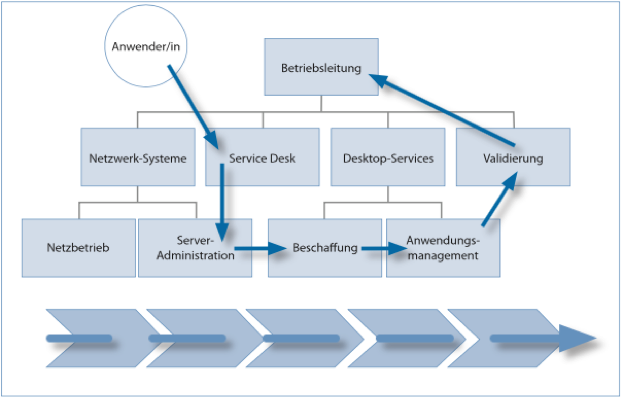
\includegraphics[width=15cm]{kapitel/gruppe1_2/bilder/aufgaben-versus_prozessorientierung} 
	\caption{Aufgaben- versus Prozessorientierung\protect\footnotemark}
	\label{fig_aufgaben_vs_prozess}
\end{figure}\footnotetext{\cite[Vgl.][35]{leitner_itil_2008}}

Die Erreichung der Prozessorientierung kann auf unterschiedliche Weise erfolgen, zum Beispiel durch 
eine kontinuierliche Prozessverbesserung oder die Gestaltung und Anpassung von IT-Strukturen 
\footcite[Vgl.][45]{wissensmanagement_2010}. Im Rahmen des Kapitels 
\ref{subsubsection_kontinuierlicher_verbesserungsprozess}  wird der in der oberen Abbildung gezeigte 
kontinuierlicher Verbesserungsprozess beschrieben, evaluiert und letztendlich optimiert.

\subsubsection{Kontinuierlicher Verbesserungsprozess}
\label{subsubsection_kontinuierlicher_verbesserungsprozess}
Das Ziel des kontinuierlichen Verbesserungsprozesses ist die stetige Verbesserung von Zuständen in 
kleinen Schritten und die Wahrung der  Zustandsverbesserung, wie in Abbildung 
\ref{fig_kontinuierliche_verbesserung} gut veranschaulicht. Zur Umsetzung systematischer 
Verbesserungsmaßnahmen, wird ein in 4. Phasen aufgeteilter Regelkreis angewandt.

\begin{figure}[h!]
	\centering
	
\includegraphics[width=5cm]{kapitel/gruppe1_2/bilder/kontinuierlicher_verbesserungsprozess} 
	\caption{Kontinuierlicher Verbesserungsprozess\protect\footnotemark}
	\label{fig_kontinuierliche_verbesserung}
\end{figure}\footnotetext{\cite{yasar_kvp_2015}}

In der Phase Plan wird sich die Frage gestellt, was und wie etwas zu tun ist. Auf die Prozessorientierung angewandt, lässt sich hier auf die Prozessdefinition und –analyse schließen. Die Phase Do beschäftigt sich mit der Frage was erreicht wurde und steht für die Ausführung, also sinnbildlich für die Prozesskonstruktion. Bei der Check-Phase geht man auf die Frage ein, was noch zu tun ist und ob die Aufgaben nach Plan erfüllt sind, ableitbar auf eine Prozessvalidierung. In der letzten Phase Act wird überprüft, welche Dinge verbessert werden können, das für eine Prozessoptimierung und –automatisierung spricht.\footcite[Vgl.]{yasar_kvp_2015}

\paragraph{Prozessidentifizierung und -analyse}\mbox{}\\\\
\label{paragraph_prozessidenifizierung}
Die Aufgabe der Prozessidentifizierung ist es, Prozesse zu bestimmen und zu beschreiben, die mit hoher Priorität geplant, gesteuert und verbessert werden sollen. In der Prozessanalyse werden dann die einzelnen Elemente eines Prozesses und deren Beziehung untereinander bestimmt und beschrieben. \footcite[Vgl.][276]{heinrich_stelzer_2011}
Angewandt auf den Prozess in der Abbildung \ref{fig_aufgaben_vs_prozess} des Kapitel \ref{subsection_prozessorientierung} kann folgendes abgeleitet werden:
Der Anwender meldet eine Störung innerhalb einer Fachapplikation wie zum Beispiel der Studierendenverwaltung dem Servicedesk der Hochschule. Dieser analysiert, beschreibt und priorisiert den eingehenden Fall. Innerhalb des First-Level-Supportes und bestehender Fehlerprotokolle/-dokumentationen wird versucht, eine Sofortlösung zu erzielen. Ist dies nicht erfolgsversprechend, wird bei einer fehlerhaften Serverkonfiguration der Server-Administrator verständigt. Dieser entdeckt bei seiner Untersuchung ein fehlendes Update der Fachapplikation und beauftragt damit die Beschaffungsabteilung. Das Einspielen des Updates wird durch das Anwendungsmanagement auf einem Testsystem durchgeführt, die sich anschließend zwecks Qualitätssicherung mit der Testgruppe zur Validierung abstimmt. Nach Freigabe durch die Betriebsleitung kann die Aktualisierung auf dem Produktivsystem eingespielt werden.
Ein in der Abbildung nicht aufgeführter möglicher Rückweg wäre: Nach Freigabe des Updates wird durch das Anwendungsmanagement die Installation auf dem Produktivsystem veranlasst. Der Servicedesk wird hierrüber nach erfolgreichem Abschluss informiert, der die Fehlerbehandlung protokolliert und den Endanwender über die Lösung der gemeldeten Störung unterrichtet.

\paragraph{Prozesskonstruktion und –sichtbarkeit}\mbox{}\\\\
\label{paragraph_prozesskonstruktion_und_sichtbarkeit}
Um die im vorherigen Kapitel bei der Prozessanalysendefinition erwähnten Elemente sichtbar zu machen, werden Prozessketten verwendet. Diese eigenen sich, um den Ablauf bestehender Prozesse und die Beziehung der einzelnen Elemente untereinander zu visualisieren. Aber nicht nur der Ist-Prozess, sondern auch der Soll-Prozess kann mittels Prozessketten modelliert werden. Zur Verfügung stehen unterschiedliche Modellierungselemente, beispielsweise ein Rechteck zur Symbolisierung einer Funktion, eine Ellipse als organisatorisches Element (Prozessstart, Prozessende) oder Pfeile, die einen Informationsfluss veranschaulichen. \footcite[Vgl.][64]{krcmar_einfuhrung_2015} Zur Steigerung der Prozesseffizienz wurden in Kapitel \ref{subsubsection_prozessoptimierung_durch_minierung_der_durchlaufzeiten} unterschiedliche Durchlaufoptimierungen aufgeführt: \glqq Weglassen\grqq, \glqq Auslagern\grqq, \glqq Zusammen fassen\grqq, \glqq Parallelisieren\grqq, \glqq Verlagern\grqq, \glqq Beschleunigen\grqq, \glqq Keine Schleifen\grqq und \glqq Ergänzen\grqq.

Im Sinne des kontinuierlichen Verbesserungsprozesses und der in diesem Kapitel verwiesenen Prozesskonstruktion wurde im Anhang in der Abbildung \ref{fig_prozessoptimierung_gesamt} der im Kapitel \ref{paragraph_prozessidenifizierung} beschriebene Prozess der Fehlerbehandlung einer Fachapplikation mittels Prozesskette abgebildet. In der Zeilenbeschreibung sind die Zuständigen der jeweiligen Aufgaben aufgeführt. Der Prozess startet in der ersten Zeile bei „Start“ und ist der vorgegebenen Pfeilrichtung entsprechend zu lesen bis hin zum Prozessende.

\paragraph{Prozessevaluierung}\mbox{}\\\\
„Der wesentliche Zweck der Prozessevaluierung besteht darin, zu überprüfen, ob ein Geschäftsprozess gemäß den Vorgaben ausgeführt wird. Relevante Vorgaben können in Prozessentwürfen, Verfahrensanweisungen und Arbeitsanleitungen beschrieben sein“. \footcite[277]{heinrich_stelzer_2011} Es wird sich die Frage gestellt, ob die Prozesse so ausgeführt werden, wie sie in den Prozessmodellen beschrieben wurden und ob der Geschäftsprozess der kontinuierlichen Verbesserung unterliegt. \footcite[Vgl.][277]{heinrich_stelzer_2011} In unserem Beispiel wurde die Prozessmodellierung auf Basis der Prozessbeschreibung erstellt, wodurch die Prozessevaluierung positiv abschließt. Diese Evaluierung muss natürlich in regelmäßigen Abständen wiederholt werden, um zu überprüfen, ob der Gesamtprozess noch nach Plan läuft. Trotz positiver Bewertung kann auch unser Beispielprozess von einer Prozessoptimierung profitieren.

\paragraph{Prozessoptimierung}\mbox{}\\\\
\label{paragraph_prozessoptimierung}
Die Prozessoptimierung bezeichnet alle Maßnahmen zur Veränderung von Prozessen, um die Kosten zu senken, Durchlaufzeiten zu verkürzen, Innovationsfähigkeit zu erhöhen oder die Qualität zu steigern. \footcite[Vgl.][280]{heinrich_stelzer_2011}
Die im Kapitel \ref{paragraph_prozesskonstruktion_und_sichtbarkeit} gewonnenen Erkenntnisse zur Steigerung der Prozesseffizienz wurden auf unseren Fall angewandt und mündeten in einer optimierten Prozesskette. Dieses Kapitel konzentriert sich aufgrund der Komplexität auf den ersten Teilprozess, sprich die Meldung des Fehlers bis zur Freigabe des Updates. Der Rückweg in Form der Installation auf dem Produktivsystem und der Erfolgsmeldung an den Kunden ist der Vollständigkeit halber im Anhang in Abbildung \ref{fig_prozessoptimierung_gesamt} mit aufgeführt, ist aber nicht Bestandteil dieser Ausarbeitung.
Die erste Spalte der Abbildung \ref{fig_prozessoptimierung} zeichnet den aktuellen Ist-Zustand auf. Das Ergebnis einer Prozessoptimierung ist in der zweiten Spalte erkennbar, auf das nachfolgend weiter eingegangen wird. Damit die Innovation Einzug in der Hochschule hält, wäre eine übergreifende Service- und Programmüberwachung denkbar. Sie ermöglicht das entdecken und identifizieren von Fehlern vor der Meldung durch einen Endanwender. Parallel dazu wird ein Automatismus geschaffen, der neue Updates für alle Fachapplikationen sucht und bei Entdeckung an die übergreifende Überwachungssoftware meldet. Wird ein neues Update festgestellt, wird der Server-Administrator informiert, um die Serverkonfiguration zu prüfen. Es ist sinnvoll, seine Kompetenzen um das Einspielen von Updates für Applikationen zu erweitern. Nur spezifische Störungen innerhalb der Anwendung oder konkrete Nachfragen zur Bedienung sollten an das Anwendungsmanagement weitergeleitet werden.  Die Testgruppe prüft anhand vordefinierter Testfälle die Funktionsfähigkeit der Anwendung. Der Betriebsleiter gibt das Update nach positivem Testfeedback frei.
Um die einzelnen Maßnahmen zur Prozessoptimierung aufzugreifen, sind im Schaubild Kreise mit Zahlen aufgeführt:

\begin{enumerate}
	\item Maßnahme Weglassen: Im Optimalfall wird der Endanwender von einer Störung nichts mitbekommen
	\item Maßnahme Parallelisierung: Das Laden von Updates wird automatisiert und findet parallel zur Programmüberwachung statt. So wird eine verkürzte Durchlaufzeit erzielt, da der Server-Administrator sofort informiert und auf bereits heruntergeladene Updates zugreifen kann.
	\item Maßnahme Ergänzen: Durch die Einführung einer übergreifenden Überwachungssoftware wird ein neuer Teilprozess ergänzt.
	\item Maßnahme Zusammenführen: Der Serveradministrator prüft nicht nur Serverkonfigurationen, sondern spielt auch Updates ein
	\item Maßnahme Auslagern: Die Fachabteilung Beschaffung muss die Updates nicht mehr selbst herunterladen, ein Automatismus auf einem Server übernimmt diese Tätigkeit.
\end{enumerate}


\begin{figure}[h]
	\centering
	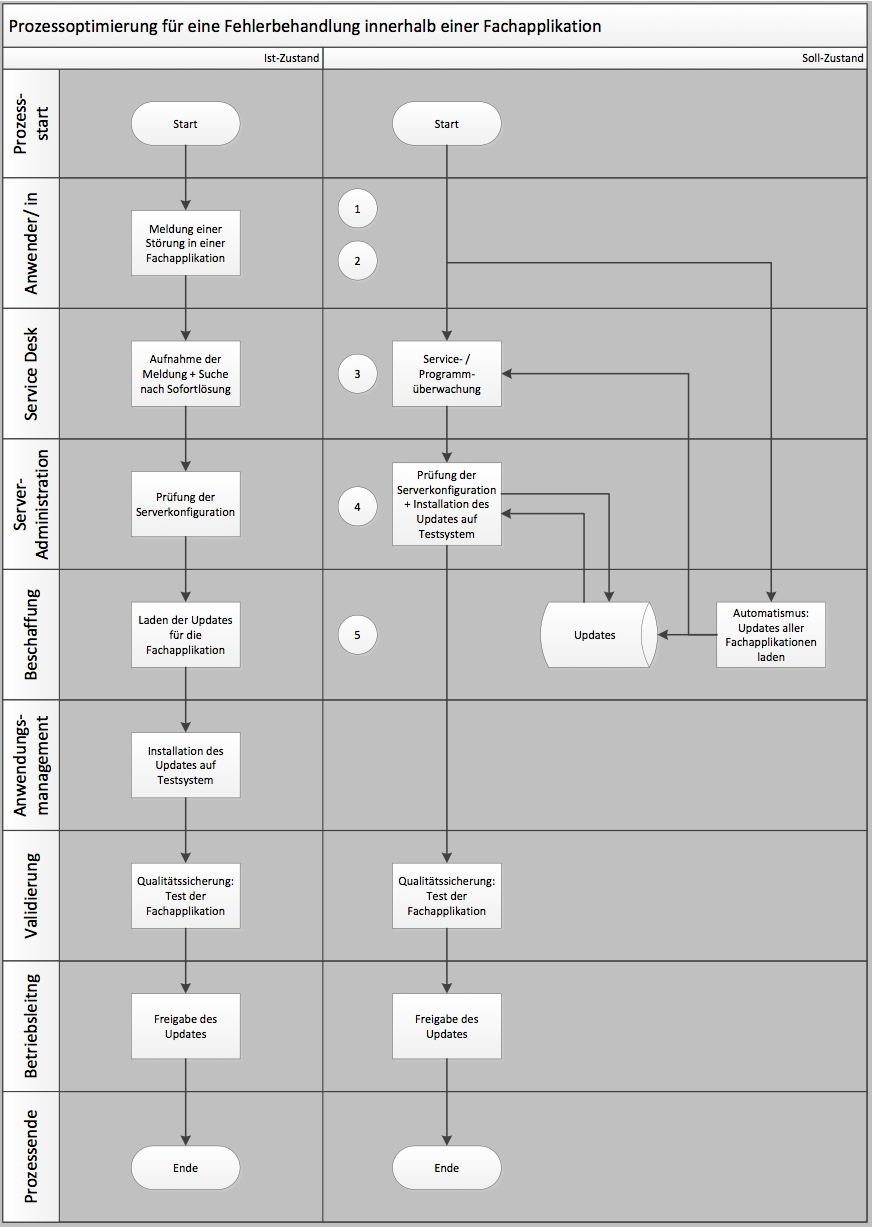
\includegraphics[width=\textwidth]{kapitel/gruppe1_2/bilder/prozessoptimierung} 
	\caption{Prozessoptimierung für eine Fehlerbehandlung}
	\label{fig_prozessoptimierung}
\end{figure}
\clearpage

\subsubsection{Gestaltung und Anpassung von IT-Strukturen}
\label{subsubsection_gestaltung_IT_strukturen}
Die Gestaltung und Anpassung von IT-Strukturen ist zur Prozessoptimierung durch Zentralisierung, Standardisierung und Outsourcing erreichbar. Wie diese Gestaltungsmaßnahmen bereits in bestehenden deutschen Hochschulen zum Einsatz kamen, erläutert Kapitel \ref{section_umsetzung_der_trends_in_den_betrachteten_hochschulen}.


\paragraph{Zentralisierung}\mbox{}\\\\
\label{paragraph_zentralisierung}
Im Hochschulbereich haben sich einige Lehrstühle und Institute ihre eigene IT-Abteilung geschaffen. Dies gilt beispielsweise für viele Leiter von Forschungsprojekten, für die Verwaltung und die Bibliothek, die eigene IT-Dienstleistungen erbringen. Das hohe Maß an Dezentralisierung der IT-Betriebsorganisationen führt zu einer Redundanz der IT-Service-Erbringung. Es ließe sich ein Parallelaufbau von betriebsrelevanter Infrastruktur wie Netz- und Stromversorgung, Belüftung und Klimatisierung vermeiden.
\footcite[Vgl.][22]{stratmann_it_2013}. Auch das doppelte Bereitstellen von beispielsweise Mailservices oder Groupware ist nicht sinnvoll. Des Weiteren wird mit diesen Standard-IT-Dienstleistungen mehrfach Personal gebunden, das mit der zunehmenden Komplexität der Basisdienstleistungen oft überfordert ist. 
Die Institute können sich nicht selbst auf allen Ebenen mit hochwertiger IT-Dienst-Betreuung befassen. Die vielen Insellösungen sind zusätzlich unwirtschaftlich und für eine hochschulweite Integration des Informationsmanagements oft hinderlich. Die Institute müssen Strategien entwickeln, um gemeinsame Synergieeffekte zu nutzen und die begrenzten IT-Betreuungsressourcen sinnvoll einzusetzen.
Die Zentralisierung von Diensten ermöglicht eine einfach zu koordinierende Beschaffung von Hard- und Software. Alle Systeme sind durch die zentrale Planung und Einbettung gut aufeinander abgestimmt und ergeben größere Ausfallsicherheit mit hoher Verfügbarkeit. Das stärkt die Stabilität und Robustheit des IT-Gesamtsystems. Die Redundanz in dem Personaleinsatz und der Serviceerbringung entfällt. \footcite[Vgl.][22]{moenkediek_2006}


\paragraph{Standardisierung}\mbox{}\\\\
\label{paragraph_standardisierung}
Unter der Standardisierung in Hochschulen wird die einheitliche Nutzung von Basisdiensten und Grundfunktionalitäten verstanden. Konkret soll die Vereinheitlichung von Anwendungsprogrammen, Prüfungsordnungen und IT-Infrastrukturen in den Fachbereichen erzielt werden. Über ein Softwareverteilungstool kann eine gleiche Version aller Applikationen sichergestellt werden. Zur Realisierung von einheitlicher IT-Infrastruktur wäre eine Zentralisierung der Serviceleistungen denkbar, wie im vorherigen Kapitel beschrieben. Die Einführung von ITIL-Standardprozessen wäre ein möglicher Weg der Umsetzung und mittels SLAs könnten auch die Reaktionszeiten auf Fehlermeldungen festgelegt werden. Ein Informationsmanager (siehe Kapitel \ref{subsubsection_cio}) würde für eine kontinuierliche Einführung und Einhaltung der Standards in allen Fachbereichen Sorge tragen. Eine Zertifizierung nach standardisierten Normen (ISO 200000), wird in den kommenden Jahren ebenfalls an Bedeutung gewinnen.\footcite[Vgl.][168]{breiter_implementierung_2011}


\paragraph{Outsourcing}\mbox{}\\\\
\label{paragraph_outsourcing}
Outsourcing besteht aus den Wörtern \glqq Outside\grqq{}, \glqq Ressource\grqq{} und \glqq Using\grqq{}. Gemeint ist damit, dass einzelne Aufgaben der IT, wie bspw. Infrastruktur, Applikationen, Prozesse, Personal oder gesamte IT-Aufgaben, auf Basis einer vertraglichen Vereinbarung, für einen definierten Zeitraum an einen externen Anbieter ausgelagert werden.\footcite[Vgl.][164]{krcmar_einfuhrung_2015} Konkrete Beispiele im Bereich der Informationstechnologie für Hochschulen wären der Betrieb des Rechenzentrums, der Anwendungsentwicklung oder der Telekommunikationsnetzwerke an andere Unternehmen abzugeben. Der Informationsmanager verspricht sich einen besseren Zugriff auf notwendige Ressourcen, Verlagerung möglicher Risiken und transparentere Ausgaben durch eine Kooperation mit Outsourcing-Gebern. Dagegen stehen erhöhter Koordinationsaufwand, komplizierte Vertragsgestaltungen und räumliche / zeitliche Distanz und damit fehlendes Vertrauen in den neuen Kooperationspartner.\footcite[Vgl.][195 ff.]{barthelemy_2001}

\subsection{Konklusion Serviceorientierung und Prozessorientierung}
Schlussfolgend aus der Definition der Serviceorientierung und der Prozessorientierung lässt sich ableiten, dass sich beide Orientierungen nicht ausschließen, sondern ergänzen.  Dienstleistungsorientierung bedeutet, dass die Bereitstellung von Informationssystemen als Leistung und Dienst am Kunden selbst verstanden und gesteuert wird. Genau dies ergänzt die Prozessorientierung mit optimierten Prozessen zur Erbringung dieser Leistungen. 
Die Hochschule Emden/Leer setzt beide Orientierungen ein, möchte sich aber laut dem Hochschulrechenzentrumsleiter Günter Müller in Richtung Prozessorientierung weiterentwickeln. \footcite{gunter_muller_interview} So empfiehlt es sich auf eine effektive und effiziente Gestaltung der Dienstleistungen zu konzentrieren und durch Standardisierung einheitliche Prozesse zu schaffen.